\appendix

\chapter{Experimental Material}
\begin{table}[ht]
    \centering
    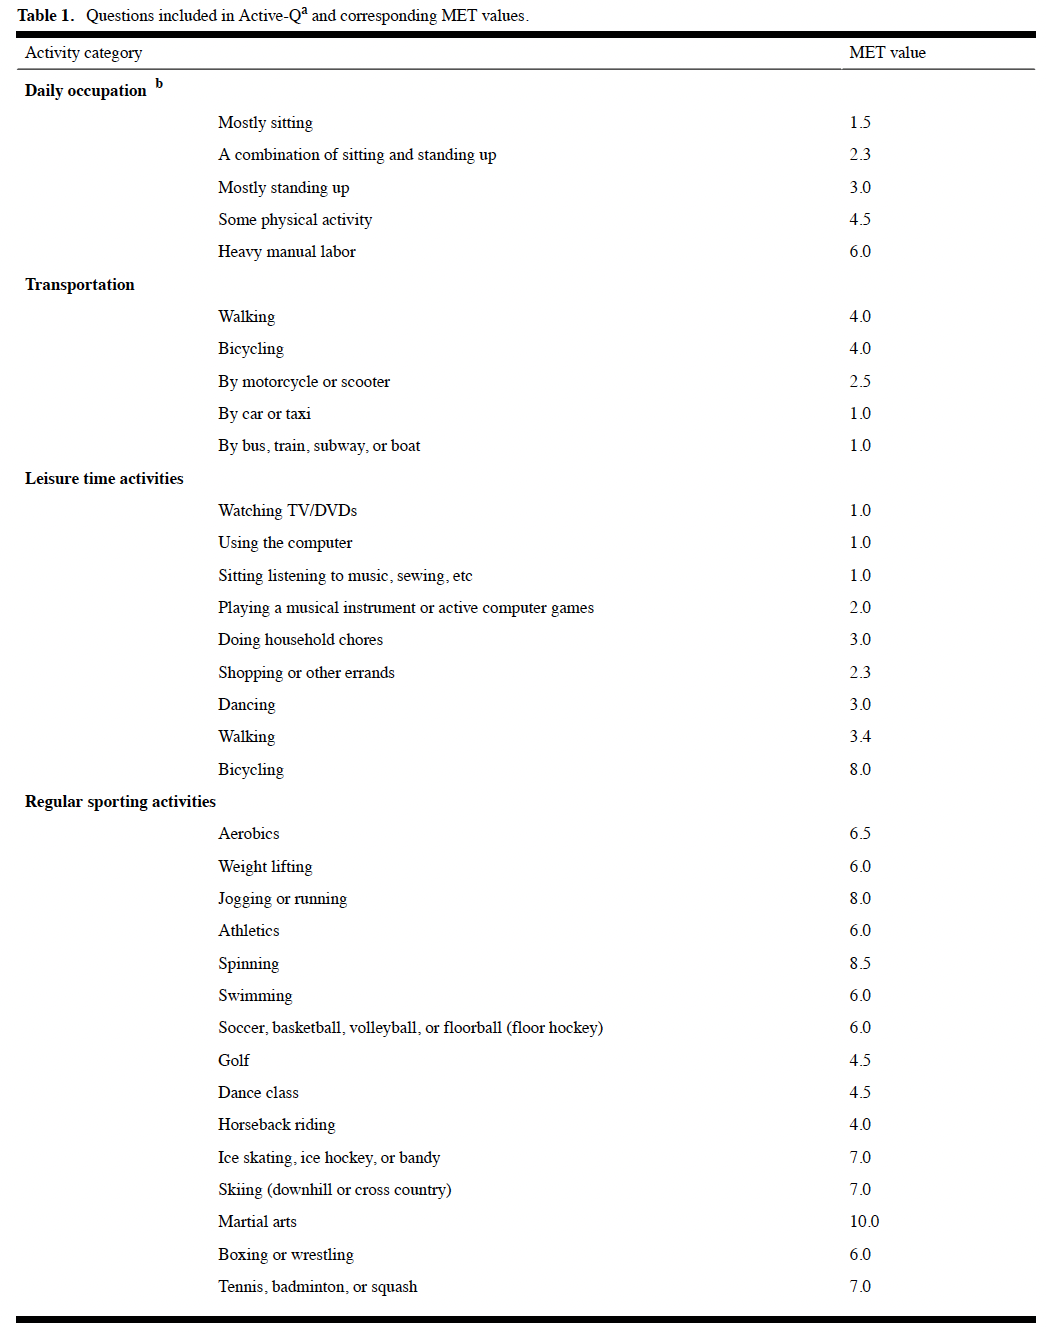
\includegraphics[width=0.8\textwidth]{appendix/met_values.png}
    \caption{MET value labels \parencite{Bonn_2012}}
    \label{tab: met_values}
\end{table}
\begin{table}[ht]
    \centering
    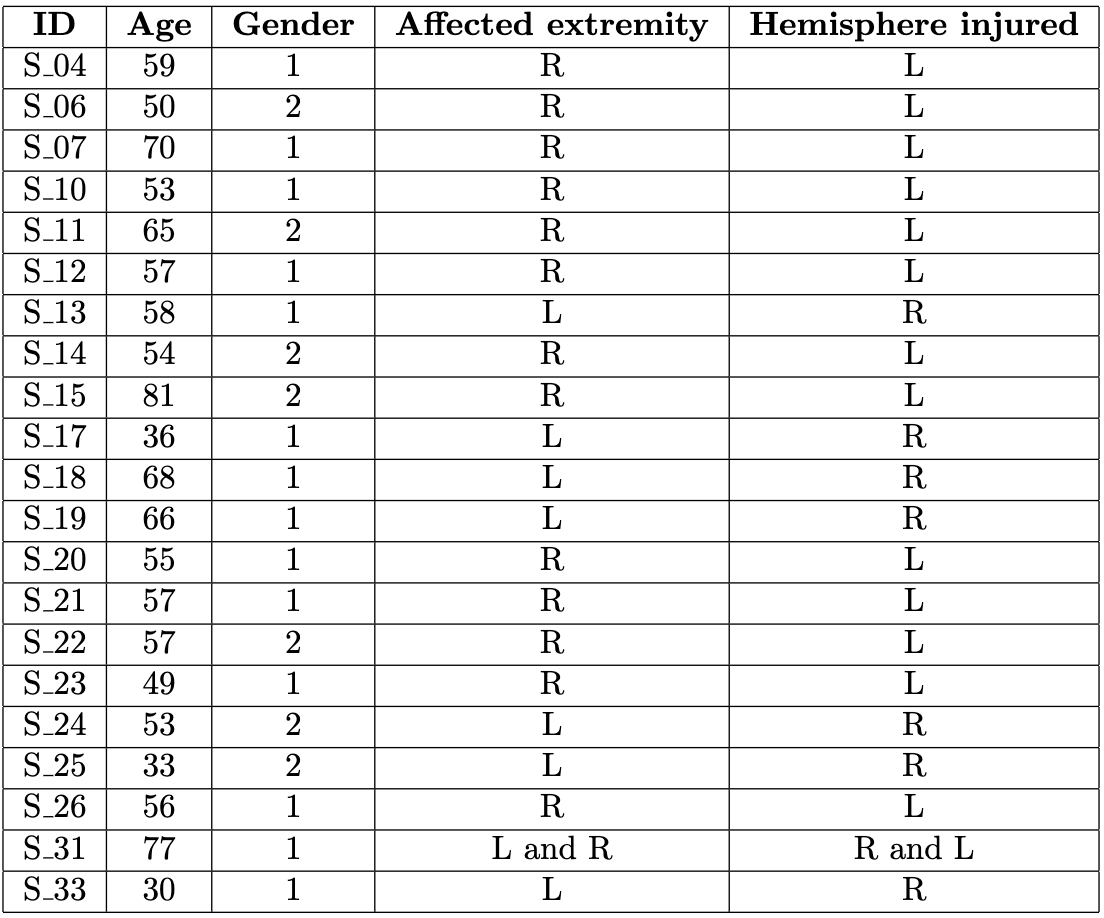
\includegraphics[width=0.70\textwidth]{appendix/database_stroke.png}
    \caption{Database for stroke population (Gender: 1 = man; 2 = woman; Hemispheres: R = right; L = left) }
    \label{tab: Database stroke}
\end{table}

\clearpage
\includepdf[scale=0.8, pages=1, 
    pagecommand={\section{Active-Q questionnaire}\label{pdf: Active-Q questionnaire}}]{appendix/Active-Q test.pdf}
\includepdf[scale=0.8, pages=2-, 
    pagecommand={}]{appendix/Active-Q test.pdf}
